% Options for packages loaded elsewhere
\PassOptionsToPackage{unicode}{hyperref}
\PassOptionsToPackage{hyphens}{url}
%
\documentclass[
  a4paper,
]{article}
\usepackage{amsmath,amssymb}
\usepackage{setspace}
\usepackage{iftex}
\ifPDFTeX
  \usepackage[T1]{fontenc}
  \usepackage[utf8]{inputenc}
  \usepackage{textcomp} % provide euro and other symbols
\else % if luatex or xetex
  \usepackage{unicode-math} % this also loads fontspec
  \defaultfontfeatures{Scale=MatchLowercase}
  \defaultfontfeatures[\rmfamily]{Ligatures=TeX,Scale=1}
\fi
\usepackage{lmodern}
\ifPDFTeX\else
  % xetex/luatex font selection
\fi
% Use upquote if available, for straight quotes in verbatim environments
\IfFileExists{upquote.sty}{\usepackage{upquote}}{}
\IfFileExists{microtype.sty}{% use microtype if available
  \usepackage[]{microtype}
  \UseMicrotypeSet[protrusion]{basicmath} % disable protrusion for tt fonts
}{}
\makeatletter
\@ifundefined{KOMAClassName}{% if non-KOMA class
  \IfFileExists{parskip.sty}{%
    \usepackage{parskip}
  }{% else
    \setlength{\parindent}{0pt}
    \setlength{\parskip}{6pt plus 2pt minus 1pt}}
}{% if KOMA class
  \KOMAoptions{parskip=half}}
\makeatother
\usepackage{xcolor}
\usepackage[margin=1in]{geometry}
\usepackage{color}
\usepackage{fancyvrb}
\newcommand{\VerbBar}{|}
\newcommand{\VERB}{\Verb[commandchars=\\\{\}]}
\DefineVerbatimEnvironment{Highlighting}{Verbatim}{commandchars=\\\{\}}
% Add ',fontsize=\small' for more characters per line
\usepackage{framed}
\definecolor{shadecolor}{RGB}{248,248,248}
\newenvironment{Shaded}{\begin{snugshade}}{\end{snugshade}}
\newcommand{\AlertTok}[1]{\textcolor[rgb]{0.94,0.16,0.16}{#1}}
\newcommand{\AnnotationTok}[1]{\textcolor[rgb]{0.56,0.35,0.01}{\textbf{\textit{#1}}}}
\newcommand{\AttributeTok}[1]{\textcolor[rgb]{0.13,0.29,0.53}{#1}}
\newcommand{\BaseNTok}[1]{\textcolor[rgb]{0.00,0.00,0.81}{#1}}
\newcommand{\BuiltInTok}[1]{#1}
\newcommand{\CharTok}[1]{\textcolor[rgb]{0.31,0.60,0.02}{#1}}
\newcommand{\CommentTok}[1]{\textcolor[rgb]{0.56,0.35,0.01}{\textit{#1}}}
\newcommand{\CommentVarTok}[1]{\textcolor[rgb]{0.56,0.35,0.01}{\textbf{\textit{#1}}}}
\newcommand{\ConstantTok}[1]{\textcolor[rgb]{0.56,0.35,0.01}{#1}}
\newcommand{\ControlFlowTok}[1]{\textcolor[rgb]{0.13,0.29,0.53}{\textbf{#1}}}
\newcommand{\DataTypeTok}[1]{\textcolor[rgb]{0.13,0.29,0.53}{#1}}
\newcommand{\DecValTok}[1]{\textcolor[rgb]{0.00,0.00,0.81}{#1}}
\newcommand{\DocumentationTok}[1]{\textcolor[rgb]{0.56,0.35,0.01}{\textbf{\textit{#1}}}}
\newcommand{\ErrorTok}[1]{\textcolor[rgb]{0.64,0.00,0.00}{\textbf{#1}}}
\newcommand{\ExtensionTok}[1]{#1}
\newcommand{\FloatTok}[1]{\textcolor[rgb]{0.00,0.00,0.81}{#1}}
\newcommand{\FunctionTok}[1]{\textcolor[rgb]{0.13,0.29,0.53}{\textbf{#1}}}
\newcommand{\ImportTok}[1]{#1}
\newcommand{\InformationTok}[1]{\textcolor[rgb]{0.56,0.35,0.01}{\textbf{\textit{#1}}}}
\newcommand{\KeywordTok}[1]{\textcolor[rgb]{0.13,0.29,0.53}{\textbf{#1}}}
\newcommand{\NormalTok}[1]{#1}
\newcommand{\OperatorTok}[1]{\textcolor[rgb]{0.81,0.36,0.00}{\textbf{#1}}}
\newcommand{\OtherTok}[1]{\textcolor[rgb]{0.56,0.35,0.01}{#1}}
\newcommand{\PreprocessorTok}[1]{\textcolor[rgb]{0.56,0.35,0.01}{\textit{#1}}}
\newcommand{\RegionMarkerTok}[1]{#1}
\newcommand{\SpecialCharTok}[1]{\textcolor[rgb]{0.81,0.36,0.00}{\textbf{#1}}}
\newcommand{\SpecialStringTok}[1]{\textcolor[rgb]{0.31,0.60,0.02}{#1}}
\newcommand{\StringTok}[1]{\textcolor[rgb]{0.31,0.60,0.02}{#1}}
\newcommand{\VariableTok}[1]{\textcolor[rgb]{0.00,0.00,0.00}{#1}}
\newcommand{\VerbatimStringTok}[1]{\textcolor[rgb]{0.31,0.60,0.02}{#1}}
\newcommand{\WarningTok}[1]{\textcolor[rgb]{0.56,0.35,0.01}{\textbf{\textit{#1}}}}
\usepackage{graphicx}
\makeatletter
\def\maxwidth{\ifdim\Gin@nat@width>\linewidth\linewidth\else\Gin@nat@width\fi}
\def\maxheight{\ifdim\Gin@nat@height>\textheight\textheight\else\Gin@nat@height\fi}
\makeatother
% Scale images if necessary, so that they will not overflow the page
% margins by default, and it is still possible to overwrite the defaults
% using explicit options in \includegraphics[width, height, ...]{}
\setkeys{Gin}{width=\maxwidth,height=\maxheight,keepaspectratio}
% Set default figure placement to htbp
\makeatletter
\def\fps@figure{htbp}
\makeatother
\setlength{\emergencystretch}{3em} % prevent overfull lines
\providecommand{\tightlist}{%
  \setlength{\itemsep}{0pt}\setlength{\parskip}{0pt}}
\setcounter{secnumdepth}{-\maxdimen} % remove section numbering
\ifLuaTeX
\usepackage[bidi=basic]{babel}
\else
\usepackage[bidi=default]{babel}
\fi
\babelprovide[main,import]{catalan}
% get rid of language-specific shorthands (see #6817):
\let\LanguageShortHands\languageshorthands
\def\languageshorthands#1{}
\ifLuaTeX
  \usepackage{selnolig}  % disable illegal ligatures
\fi
\usepackage{bookmark}
\IfFileExists{xurl.sty}{\usepackage{xurl}}{} % add URL line breaks if available
\urlstyle{same}
\hypersetup{
  pdftitle={U5. LUBUNTU. INSTAL·LACIÓ I ESTRUCTURA},
  pdfauthor={@tofermos 2024},
  pdflang={ca-ES},
  hidelinks,
  pdfcreator={LaTeX via pandoc}}

\title{U5. LUBUNTU. INSTAL·LACIÓ I ESTRUCTURA}
\usepackage{etoolbox}
\makeatletter
\providecommand{\subtitle}[1]{% add subtitle to \maketitle
  \apptocmd{\@title}{\par {\large #1 \par}}{}{}
}
\makeatother
\subtitle{Preparar un Pendrive amb Ventoy}
\author{@tofermos 2024}
\date{}

\begin{document}
\maketitle

{
\setcounter{tocdepth}{2}
\tableofcontents
}
\setstretch{1.5}
El Ventoy és una utilitat per a preparar un Pendrive. Una vegada
instal·lada al Pen, podrem usar-lo per instal·lar el SO que vullguem.
Només caldrà copiar la ISO del SO al Pen (tantes com càpiguen !)

\newpage
\renewcommand\tablename{Tabla}

\section{1. Preparar un Ventoy amb una
ISO.}\label{preparar-un-ventoy-amb-una-iso.}

\subsection{1.1. Descarregar Ventoy}\label{descarregar-ventoy}

\begin{enumerate}
\def\labelenumi{\arabic{enumi}.}
\tightlist
\item
  Accedeix a la pàgina oficial de Ventoy: \url{https://www.ventoy.net}.
\item
  Descarrega el fitxer per a Linux (\texttt{ventoy-x.x.x-linux.tar.gz}).
\end{enumerate}

\begin{figure}
\centering
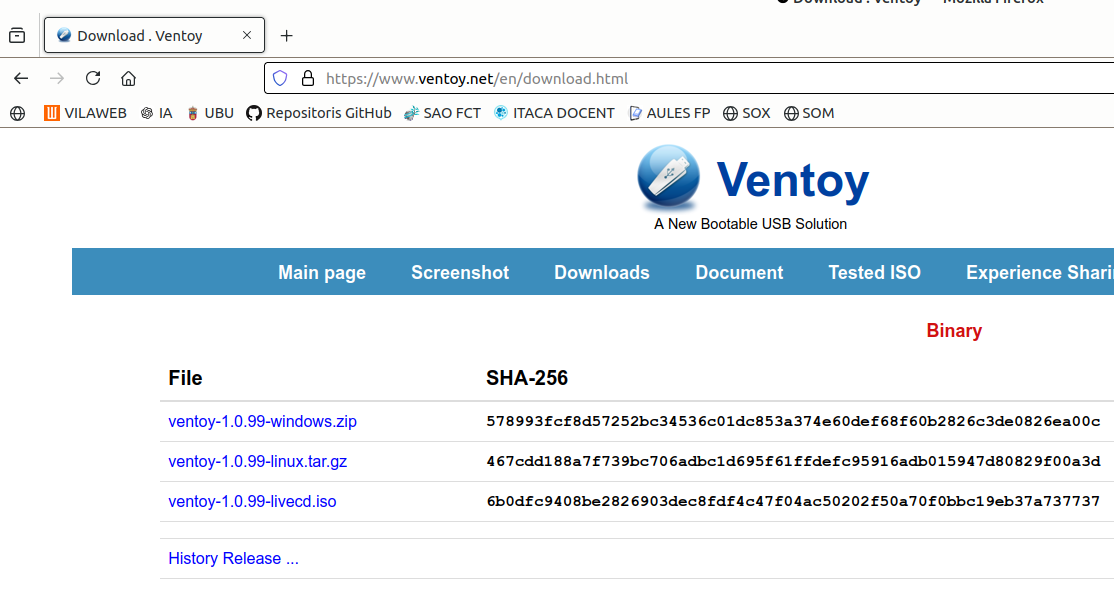
\includegraphics{png/DescarregaVentoy.png}
\caption{\emph{Figura 1: Descàrrega del Ventoy}}
\end{figure}

\subsection{1.2 Descomprimir i
instal·lar}\label{descomprimir-i-installar}

\begin{enumerate}
\def\labelenumi{\arabic{enumi}.}
\item
  \textbf{Obre el terminal}: Prem \texttt{Ctrl} + \texttt{Alt} +
  \texttt{T}.
\item
  \textbf{Canvia al directori de descàrregues}:

\begin{Shaded}
\begin{Highlighting}[]
\BuiltInTok{cd}\NormalTok{ \textasciitilde{}/Baixades}
\end{Highlighting}
\end{Shaded}
\item
  \textbf{Extreu el fitxer descarregat}:

\begin{Shaded}
\begin{Highlighting}[]
\FunctionTok{tar} \AttributeTok{{-}xzf}\NormalTok{ ventoy{-}x.x.x{-}linux.tar.gz}
\end{Highlighting}
\end{Shaded}

  Això crearà una carpeta amb el nom \texttt{ventoy-x.x.x}.
\item
  \textbf{Entra al directori extret}:

\begin{Shaded}
\begin{Highlighting}[]
\BuiltInTok{cd}\NormalTok{ ventoy{-}x.x.x}
\end{Highlighting}
\end{Shaded}
\end{enumerate}

\section{2 Instal·lar}\label{installar}

\subsection{2.1 Connecta el pendrive}\label{connecta-el-pendrive}

\begin{enumerate}
\def\labelenumi{\arabic{enumi}.}
\item
  Connecta el pendrive que vols preparar.
\item
  Identifica el dispositiu del pendrive al sistema:

\begin{Shaded}
\begin{Highlighting}[]
\ExtensionTok{lsblk}
\end{Highlighting}
\end{Shaded}

  Localitza el dispositiu que correspon al pendrive (exemple:
  \texttt{/dev/sda}). Assegura't d'identificar-lo correctament.
\end{enumerate}

\textbf{ATENCIÓ}: Assegura't de seleccionar el dispositiu correcte
perquè aquest procés esborrarà totes les dades del pendrive.

\subsubsection{Exemple:}\label{exemple}

\begin{figure}
\centering
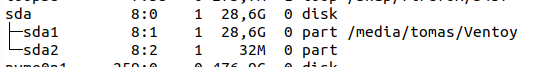
\includegraphics{png/sda.png}
\caption{\emph{Figura 2: exemple de pendrive}}
\end{figure}

\begin{center}\rule{0.5\linewidth}{0.5pt}\end{center}

\section{2.2 Instal·lar Ventoy al
pendrive}\label{installar-ventoy-al-pendrive}

Per instal·lar Ventoy al pendrive, executa:

\begin{Shaded}
\begin{Highlighting}[]
\FunctionTok{sudo}\NormalTok{ ./Ventoy2Disk.sh }\AttributeTok{{-}i}\NormalTok{ /dev/sdX}
\end{Highlighting}
\end{Shaded}

Substitueix \texttt{/dev/sdX} pel nom correcte del dispositiu del
pendrive (per exemple, \texttt{/dev/sdb}).

Durant la instal·lació, el terminal et demanarà confirmació. Escriu
\texttt{y} per continuar.

\begin{center}\rule{0.5\linewidth}{0.5pt}\end{center}

** Ja tenim el Ventoy instal·lat !**

\section{3. Copia d'arxius ISO}\label{copia-darxius-iso}

\begin{quote}
Nota: Abans de copiar la ISO podem comprovar si està correctament
descarregada.
\end{quote}

\subsection{3.1 Comprovar la ISO del SO}\label{comprovar-la-iso-del-so}

\textbf{Si la ISO està correcta, no cal fer este pas però s'ha de saber
fer.}

\subsubsection{Mirem quin codi sha256 dona el fitxer
descarregat}\label{mirem-quin-codi-sha256-dona-el-fitxer-descarregat}

A les webs de descàrregues de fitxers grans sempre torbarem un codi com
el sha256 per a fer la comporvació.

\begin{figure}
\centering
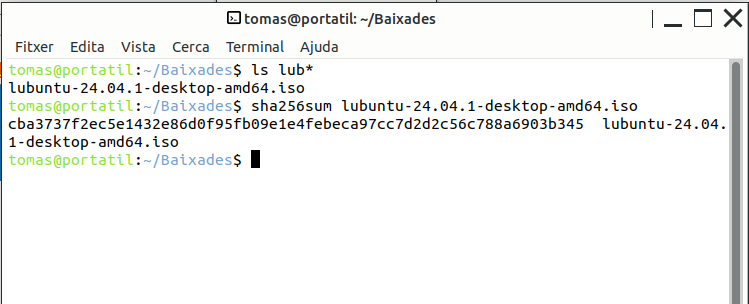
\includegraphics{png/sha256sum1.png}
\caption{*Figura 3: buscar ala web el codi sha256}
\end{figure}

\subsubsection{Busquem a la web quin codi sha256 és el
correcte}\label{busquem-a-la-web-quin-codi-sha256-uxe9s-el-correcte}

En clicar sobre l'enllaç s'obrirà un fitxer amb et codi.

\begin{figure}
\centering
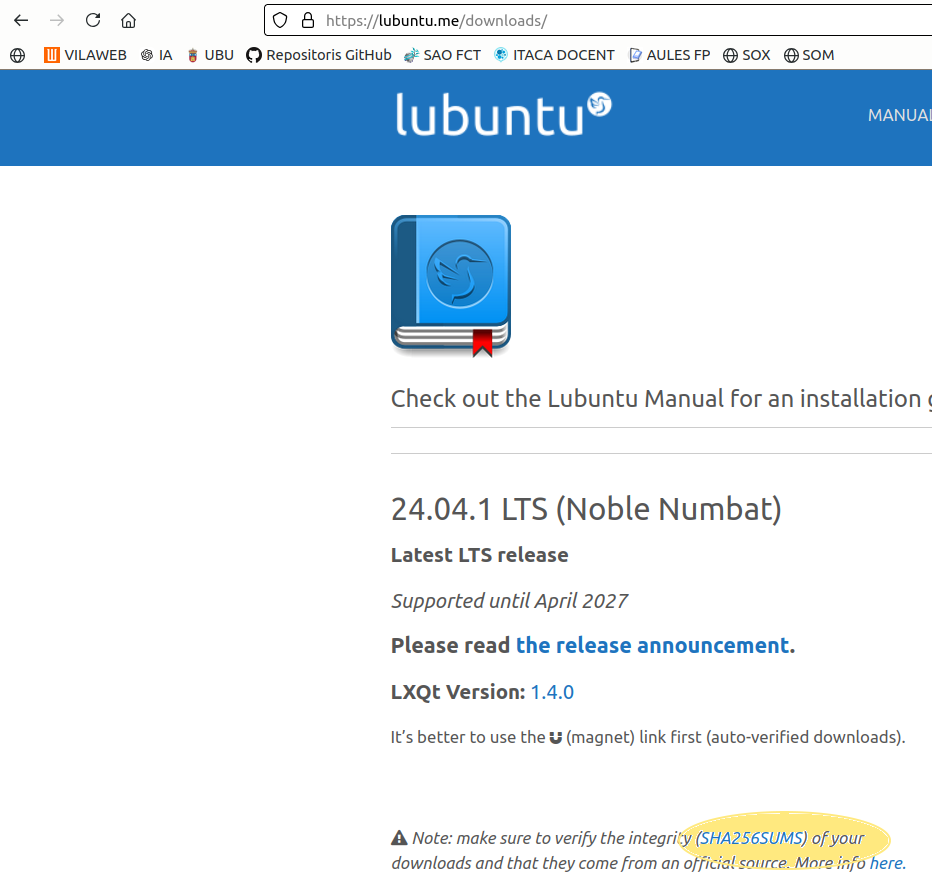
\includegraphics{png/sha256sum2.png}
\caption{\emph{Figura 4: llegir el copdi sha256}}
\end{figure}

\subsubsection{Els comparem}\label{els-comparem}

\begin{figure}
\centering
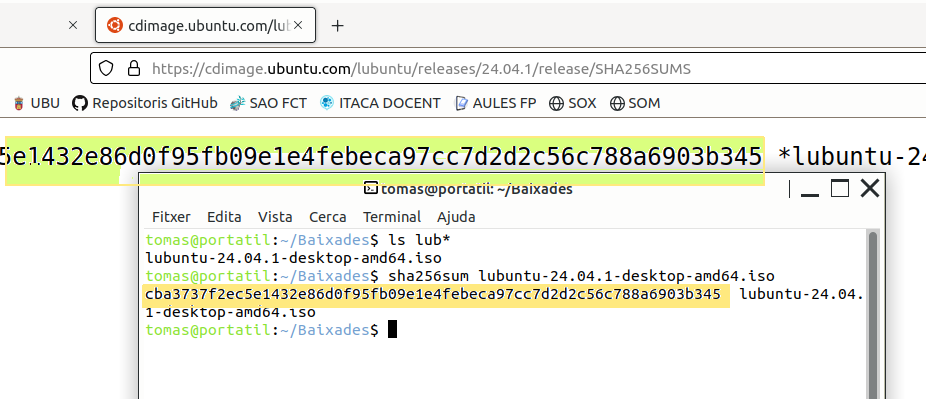
\includegraphics{png/sha256sum3.png}
\caption{\emph{Figura 3: comprovar que siguen igual}}
\end{figure}

Si el codi coindideix podem continuar\ldots{}

\subsection{3.1 Copiem les IOS que
vulguem}\label{copiem-les-ios-que-vulguem}

Una vegada instal·lat el Ventoy, el pendrive apareixerà ``buit''.

Ara pots copiar qualsevol \textbf{arxiu ISO} al pendrive i tindrem tots
els SO disponibles per instal·lar.

\section{4 Instal·lació del SO.}\label{installaciuxf3-del-so.}

Ara hem de reinciar el PC i arrancar des del Pendrive.

\begin{enumerate}
\def\labelenumi{\arabic{enumi}.}
\tightlist
\item
  Entrar a la UEFI i canviar el BootoOrder: el primer disc a buscar ha
  de ser el Pen
\item
  Insertar el pendrive i arrancar.
\item
  Ens treu un menú on triarem quin SO volem instal·lar.
\end{enumerate}

\end{document}
